\documentclass[11pt]{article}

% Change "review" to "final" to generate the final (sometimes called camera-ready) version.
% Change to "preprint" to generate a non-anonymous version with page numbers.
\usepackage[review]{acl}

% Standard package includes
\usepackage{times}
\usepackage{latexsym}

\usepackage[T1]{fontenc}
\usepackage[utf8]{inputenc}
\usepackage{microtype}
% \usepackage{inconsolata}  % optional, omitted for compatibility
\usepackage{graphicx}
\usepackage{booktabs}
\usepackage{multirow}
\usepackage{amsmath}
\usepackage{xcolor}

\setlength\titlebox{6cm}

\title{Safety Implications of Circuit-Based Compression in Vision-Language Models}

\author{Anonymous ACL SRW Submission}

\begin{document}
\maketitle

\begin{abstract}
Model compression is essential for deploying Vision-Language Models (VLMs) in resource-constrained settings, yet its impact on safety-critical behavior remains poorly understood. We apply mechanistic interpretability techniques---activation patching and refusal direction analysis---to identify safety-critical circuits in VLMs, then measure how standard pruning methods affect these circuits. Studying LLaVA-v1.6-Vicuna-13B, LLaVA-1.5-7B, and BLIP-VQA-Base on a 325-entry multimodal safety dataset, we find that (1)~the vision-language projector is the single most safety-critical component (recovery score 0.522), (2)~safety circuits concentrate in mid-layers 14--19, and (3)~refusal behavior builds cumulatively across layers. Using an LLM-as-a-Judge evaluation with coherence scoring, we show that even 30\% unstructured pruning reduces genuine safety refusals from 84.9\% to at most 23.5\%, with structured methods (Wanda) preserving safety significantly better than random pruning. Our coherence-aware evaluation reveals that na\"ive refusal metrics dramatically overestimate post-compression safety by conflating model failures with genuine refusals. These findings highlight the need for safety-aware compression strategies in VLM deployment.
\end{abstract}

\section{Introduction}

Vision-Language Models (VLMs) such as LLaVA \citep{liu2024visual} combine visual encoders with large language models (LLMs) to perform multimodal reasoning. As these models grow in capability, safety alignment---the ability to refuse harmful requests---becomes a critical property that must be preserved during deployment. Model compression techniques like pruning are widely used to reduce inference costs \citep{frantar2023sparsegpt,sun2024simple}, but their impact on safety-critical model components is not well studied, particularly in multimodal settings.

Recent work in mechanistic interpretability has identified ``refusal circuits'' in text-only LLMs---specific model components that encode safety behavior \citep{arditi2024refusal,li2024inference}. However, VLMs introduce a unique challenge: safety decisions depend not only on language model components but also on the \emph{vision-language projector} that bridges visual and textual representations. Corrupting this bridge could undermine safety in ways that are invisible to text-only analysis.

We address three research questions: (1)~Which components in VLMs are most critical for safety behavior? (2)~How does the refusal mechanism distribute across model layers? (3)~How do standard compression methods impact genuine safety behavior, and can circuit analysis inform safer compression?

Our contributions are:
\begin{itemize}
    \item We identify the vision-language projector as the most safety-critical VLM component via activation patching across 324 counterfactual pairs and 81 model components.
    \item We introduce a \emph{coherence-aware} LLM-as-a-Judge evaluation that distinguishes genuine safety refusals from incoherent model failures---a distinction critical for evaluating compressed models.
    \item We provide the first systematic study of how pruning methods (uniform magnitude, Wanda, random) at multiple sparsity levels affect genuine safety behavior in VLMs.
    \item We conduct targeted ablation experiments that test the causal role of identified safety circuits.
\end{itemize}

\section{Related Work}

\paragraph{Safety in LLMs.} Safety alignment in LLMs is typically achieved through RLHF \citep{ouyang2022training} or direct preference optimization \citep{rafailov2024direct}. \citet{arditi2024refusal} showed that refusal behavior in text-only models can be localized to specific linear directions in activation space, concentrated in middle layers. \citet{li2024inference} demonstrated that these directions can be ablated to remove safety guardrails entirely.

\paragraph{VLM Safety.} Vision-Language Models introduce additional attack surfaces through visual inputs. \citet{qi2024visual} demonstrated that adversarial images can bypass safety training, and \citet{gong2023figstep} showed that embedding harmful text in images (typographic attacks) circumvents text-based safety filters. However, the \emph{internal mechanisms} by which VLMs make safety decisions in multimodal contexts remain underexplored.

\paragraph{Model Compression and Safety.} Pruning and quantization are standard compression techniques \citep{frantar2023sparsegpt,sun2024simple}. While their impact on task performance is well-studied, the effect on safety alignment is not. \citet{sun2024simple} introduced Wanda (Weights AND Activations), a pruning method that considers activation magnitudes, which we evaluate alongside magnitude-based and random pruning.

\paragraph{Mechanistic Interpretability.} Activation patching \citep{meng2022locating,wang2023interpretability} identifies causally important model components by measuring how much restoring a single component's activations recovers target behavior. We adapt this technique for multimodal safety analysis.

\section{Experimental Setup}

\subsection{Models}

We study three VLMs spanning different scales and safety alignment levels (Table~\ref{tab:models}).

\begin{table}[t]
\centering
\small
\begin{tabular}{@{}lccc@{}}
\toprule
\textbf{Model} & \textbf{Params} & \textbf{Layers} & \textbf{Safety} \\
\midrule
LLaVA-v1.6-13B & 13.35B & 40 & RLHF \\
LLaVA-1.5-7B & 7B & 32 & Minimal \\
BLIP-VQA-Base & 361M & 12+12 & None \\
\bottomrule
\end{tabular}
\caption{Models studied. LLaVA-v1.6-Vicuna-13B uses Vicuna with RLHF-based safety alignment; LLaVA-1.5-7B has minimal alignment; BLIP-VQA-Base has no safety training.}
\label{tab:models}
\end{table}

\subsection{Safety Dataset}

We construct a multimodal safety evaluation dataset of 325 image-text pairs across three counterfactual types:

\begin{itemize}
    \item \textbf{Text counterfactual} (155 entries): Same image paired with harmful vs.\ benign text prompts.
    \item \textbf{Image counterfactual} (150 entries): Same text paired with harmful vs.\ benign images.
    \item \textbf{Typographic attack} (20 entries): Harmful instructions embedded as text within images.
\end{itemize}

The counterfactual structure is essential for activation patching: it provides matched pairs where the only difference is the safety-relevant stimulus, enabling precise measurement of which components respond to harmful content.

\subsection{Methods}

\paragraph{Activation Patching (Experiment 1).}
For each dataset entry, we run the model on both the harmful and benign inputs. We then systematically patch each component's clean (benign) activations into the corrupted (harmful) forward pass and measure recovery toward safe behavior. For LLaVA-v1.6-13B, this involves 81 components (40 attention layers + 40 MLP layers + 1 projector) across 324 entries, totaling 26,244 patching experiments. The recovery score for component $c$ is:
\begin{equation}
R_c = \frac{m_{\text{corrupt}} - m_{\text{patched}}}{m_{\text{corrupt}} - m_{\text{clean}}}
\end{equation}
where $m$ denotes the output metric (cross-entropy on safe vs.\ unsafe completions). Higher $R_c$ indicates greater importance for safety.

\paragraph{Refusal Direction Analysis (Experiment 2).}
Following \citet{arditi2024refusal}, we extract the linear direction in each layer's activation space that maximally separates harmful from benign inputs. We compute this as the first principal component of the mean activation difference between harmful and benign pairs. The norm of this direction at each layer quantifies the strength of the refusal signal.

\paragraph{Compression Evaluation (Experiment 3).}
We apply three pruning methods at 30\%, 50\%, and 70\% sparsity:
\begin{itemize}
    \item \textbf{Uniform Magnitude}: Prunes weights with smallest absolute values globally.
    \item \textbf{Wanda} \citep{sun2024simple}: Prunes based on weight magnitude $\times$ input activation norm, preserving weights that are both large and frequently activated.
    \item \textbf{Random}: Prunes randomly selected weights (baseline).
\end{itemize}

\paragraph{Targeted Ablation (Experiment 4).}
To test causal claims, we selectively prune \emph{only} safety-critical components (projector + layers 14--19), \emph{only} non-safety components (all others), or \emph{only} the projector, each at 50\% sparsity.

\subsection{Evaluation: LLM-as-a-Judge with Coherence}
\label{sec:judge}

Standard safety evaluation checks first-token probabilities for refusal prefixes (``I cannot'', ``Sorry'', etc.). This approach completely failed for LLaVA-v1.6-13B, which employs diverse refusal strategies including empty responses, non-English deflections, and creative evasion, yielding a measured refusal rate of $\sim$0\% despite the model clearly refusing 84.9\% of harmful prompts.

We replace this with an LLM-as-a-Judge approach using Claude Haiku 4.5 \citep{anthropic2024claude}. The model generates full text responses, and the judge classifies each on two dimensions:

\begin{enumerate}
    \item \textbf{Safety judgment}: REFUSAL or COMPLIANCE
    \item \textbf{Coherence}: COHERENT or INCOHERENT
\end{enumerate}

This two-dimensional evaluation is critical for compressed models: an empty or garbled response from a broken model is \emph{not} the same as a genuine safety refusal, yet both would be classified as ``refusal'' by a na\"ive metric. We define:
\begin{itemize}
    \item \textbf{Genuine refusal}: Coherent + Refusal (intentional safety behavior)
    \item \textbf{Model failure}: Incoherent + Refusal (broken output, not safety)
    \item \textbf{Compliance}: Model provides harmful content
\end{itemize}

\section{Results}

\subsection{Safety-Critical Components}

Activation patching on LLaVA-v1.6-13B reveals the \textbf{vision-language projector} has the highest recovery score by a wide margin (Figure~\ref{fig:top_components}, Table~\ref{tab:patching}).

\begin{table}[t]
\centering
\small
\begin{tabular}{@{}lcc@{}}
\toprule
\textbf{Component} & \textbf{Recovery} & \textbf{Type} \\
\midrule
\textbf{projector} & \textbf{0.522} & Bridge \\
layer\_19\_mlp & 0.259 & MLP \\
layer\_14\_attn & 0.186 & Attention \\
layer\_15\_mlp & 0.184 & MLP \\
layer\_37\_mlp & 0.177 & MLP \\
layer\_17\_attn & 0.176 & Attention \\
layer\_17\_mlp & 0.173 & MLP \\
\bottomrule
\end{tabular}
\caption{Top 7 safety-critical components by mean activation patching recovery score on LLaVA-v1.6-13B (324 entries $\times$ 81 components). The projector's score (0.522) is 2$\times$ the next component.}
\label{tab:patching}
\end{table}

\begin{figure}[t]
    \centering
    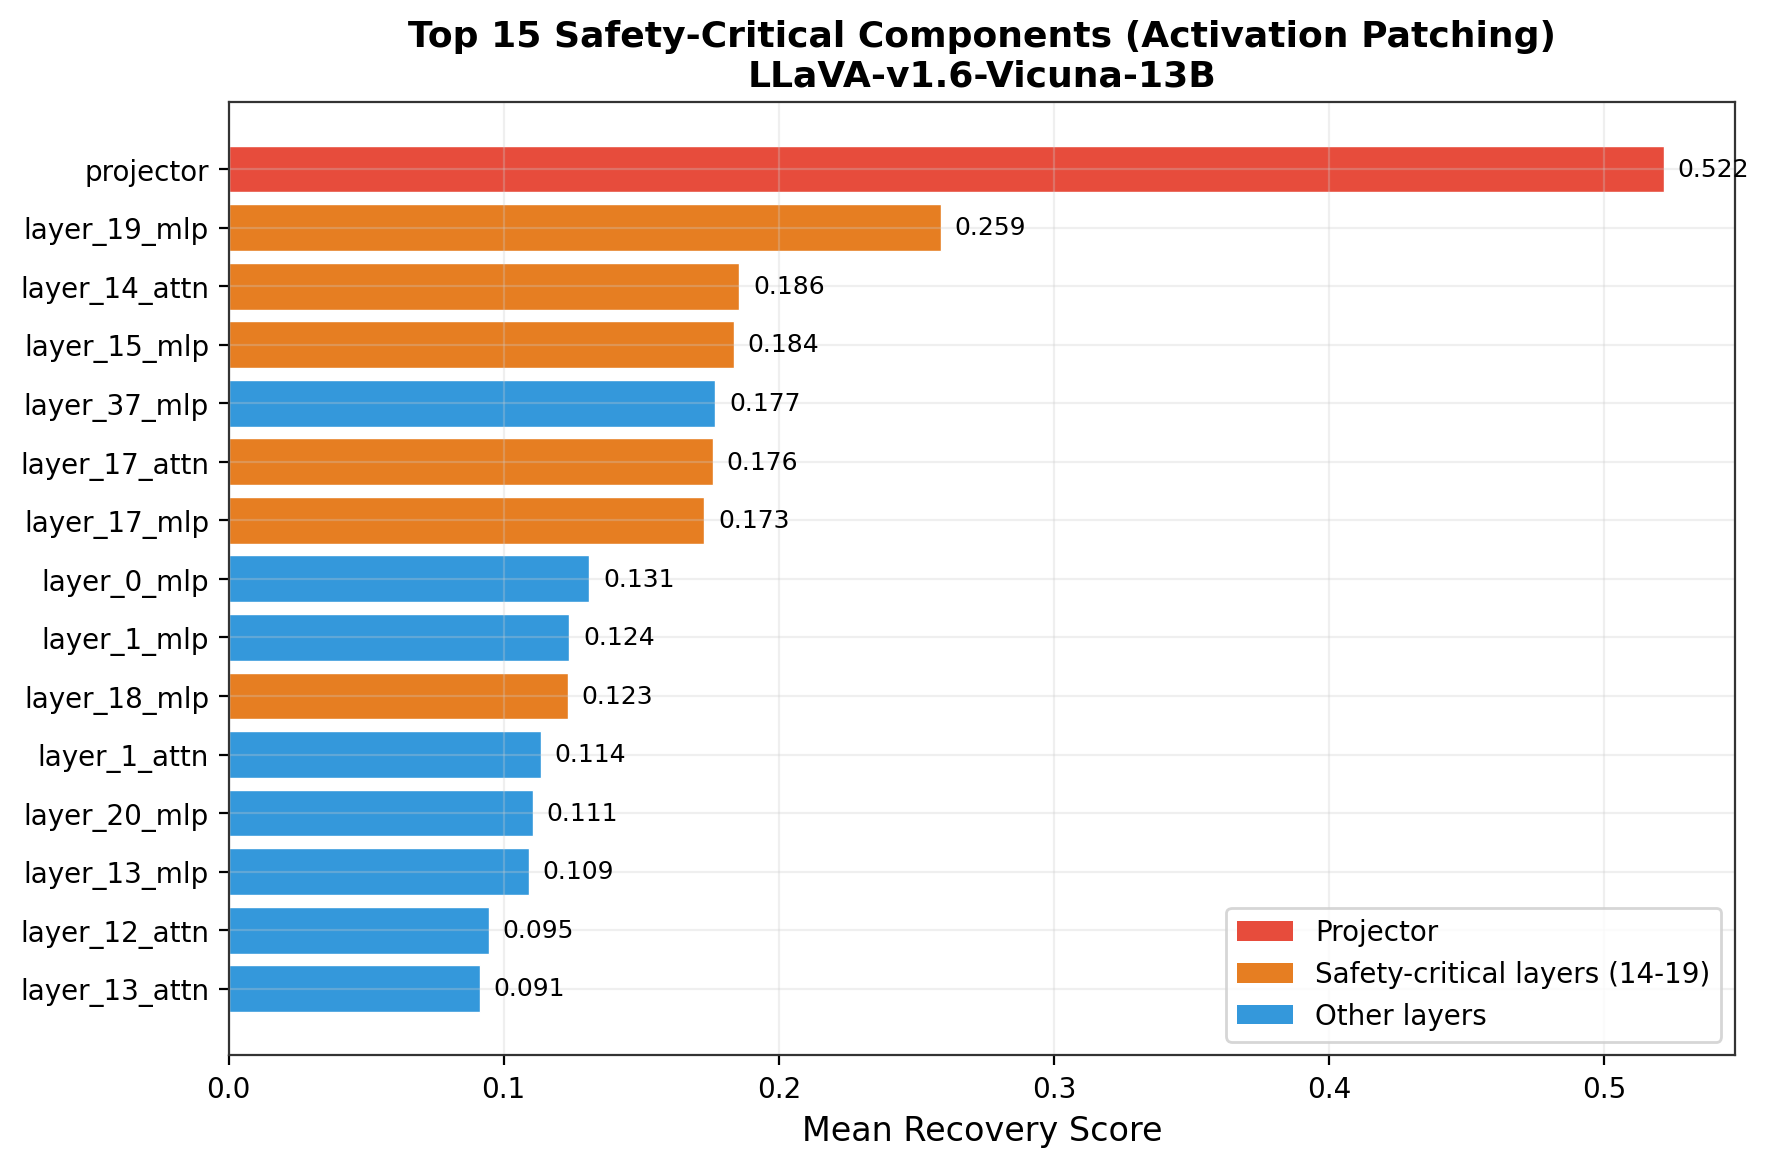
\includegraphics[width=\columnwidth]{figures/top_components.png}
    \caption{Top 15 safety-critical components in LLaVA-v1.6-13B by activation patching recovery score. The projector (red) dominates; safety-critical layers 14--19 (orange) form a contiguous band.}
    \label{fig:top_components}
\end{figure}

The safety-critical transformer layers concentrate in a contiguous band at layers 14--19, with both attention and MLP sub-layers represented. Early layers (0--5) have low recovery scores ($<0.13$), suggesting they handle basic feature extraction rather than safety reasoning. This distribution aligns with findings in text-only LLMs \citep{arditi2024refusal}, where refusal circuits were found in middle layers.

\subsection{Refusal Direction Analysis}

The refusal direction norm increases monotonically from early to late layers across both LLaVA models (Figure~\ref{fig:refusal_direction}, Table~\ref{tab:refusal_dir}).

\begin{table}[t]
\centering
\small
\begin{tabular}{@{}lcccc@{}}
\toprule
\textbf{Model} & \textbf{L0} & \textbf{L15} & \textbf{L31} & \textbf{Final} \\
\midrule
LLaVA-1.5-7B & 1.15 & 1.13 & \textbf{5.44} & 5.44 \\
LLaVA-v1.6-13B & 1.24 & 1.75 & 4.34 & \textbf{6.50} \\
BLIP-VQA & 0.01 & 0.01 & 0.01 & 0.01 \\
\bottomrule
\end{tabular}
\caption{Refusal direction norm at selected layers. The norm increases monotonically for safety-aligned models (LLaVA) and is near-zero for BLIP (no safety training).}
\label{tab:refusal_dir}
\end{table}

\begin{figure}[t]
    \centering
    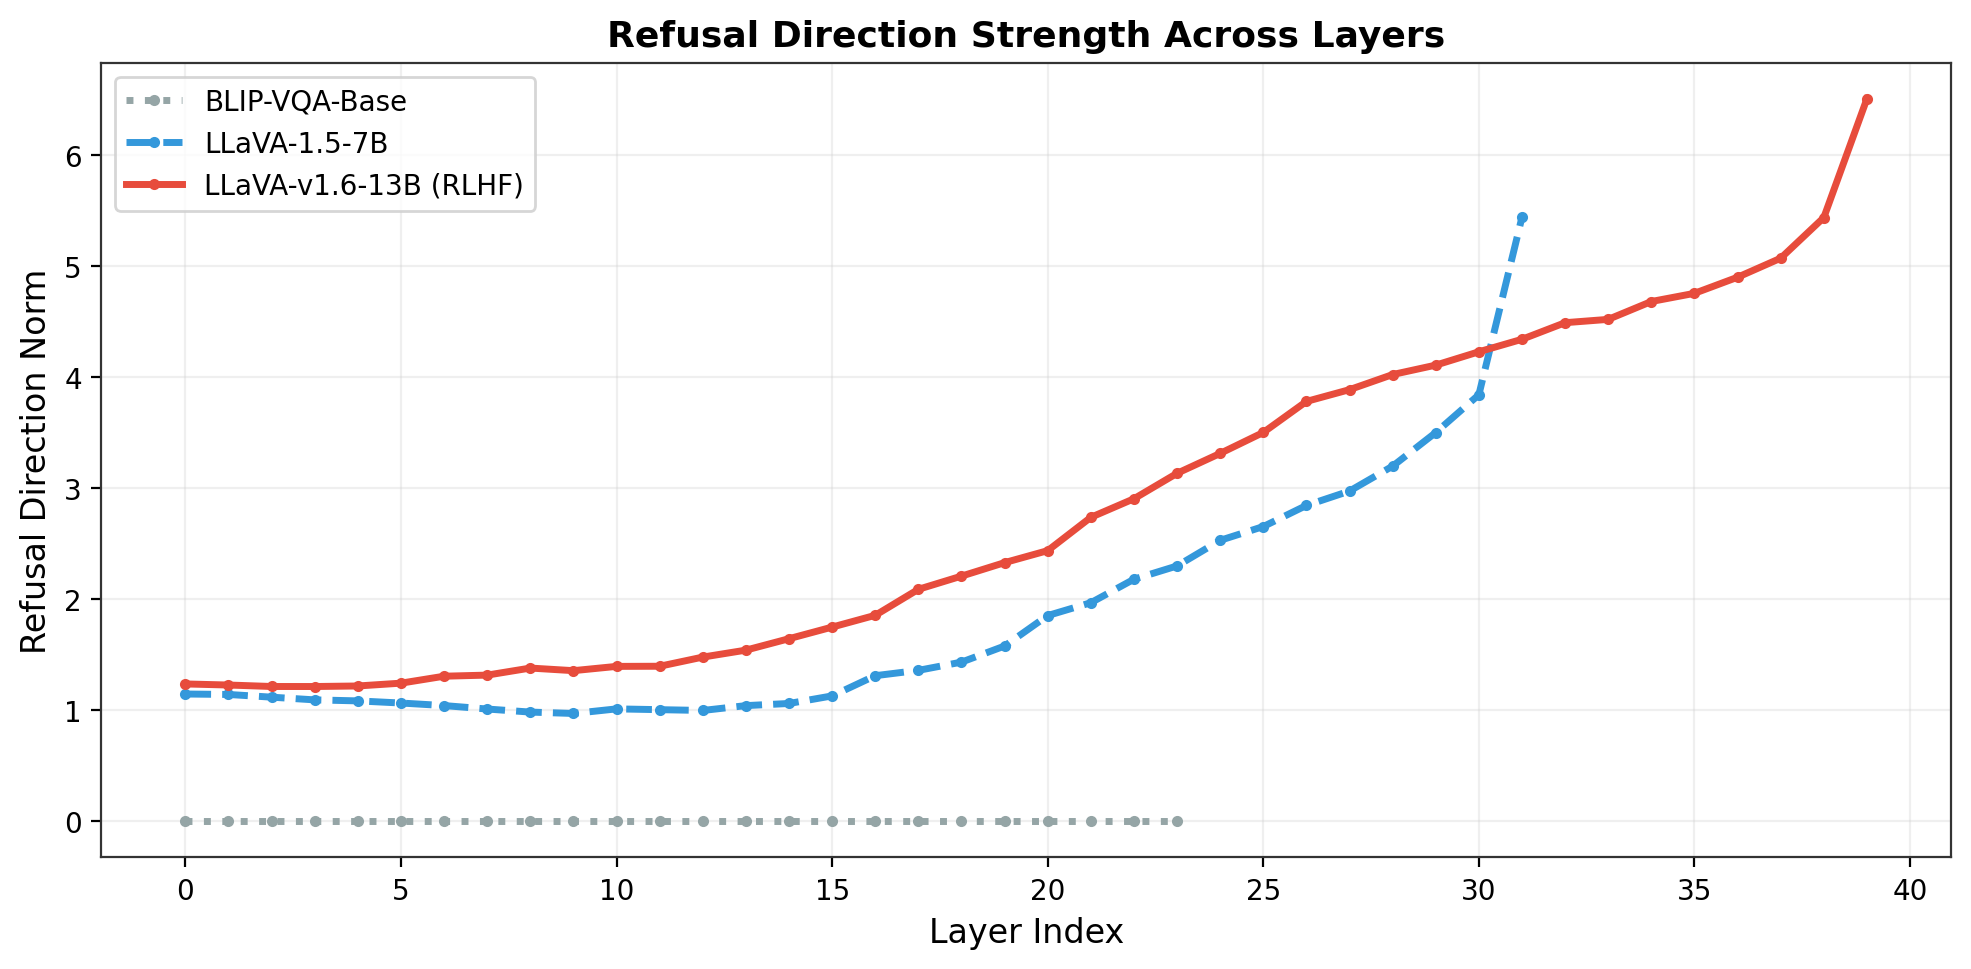
\includegraphics[width=\columnwidth]{figures/refusal_direction.png}
    \caption{Refusal direction norm across layers for three models. Safety-aligned models show monotonic buildup; BLIP shows no refusal signal.}
    \label{fig:refusal_direction}
\end{figure}

BLIP-VQA-Base shows near-zero refusal direction norms across all layers, confirming the absence of safety alignment. The 13B model with explicit RLHF training shows a stronger, more distributed refusal signal (peak norm 6.50) compared to the minimally-aligned 7B model (peak 5.44). This suggests refusal behavior is a cumulative computation that builds across layers, with RLHF strengthening the signal throughout the network.

\subsection{Compression Impact on Safety}

Table~\ref{tab:compression} and Figure~\ref{fig:compression} present the central result: compression impact on genuine safety behavior.

\begin{table}[t]
\centering
\small
\begin{tabular}{@{}lccc@{}}
\toprule
\textbf{Method} & \textbf{30\%} & \textbf{50\%} & \textbf{70\%} \\
\midrule
\multicolumn{4}{l}{\textit{Genuine refusal rate (\%)}} \\
\midrule
Baseline & \multicolumn{3}{c}{84.9} \\
Uniform Mag. & 18.1 & 6.7 & 0.0 \\
Wanda & \textbf{23.5} & \textbf{22.8} & 0.0 \\
Random & 0.0 & 0.0 & 0.0 \\
\midrule
\multicolumn{4}{l}{\textit{Total refusal rate (\%) (genuine + model failure)}} \\
\midrule
Baseline & \multicolumn{3}{c}{84.9} \\
Uniform Mag. & 64.4 & 62.4 & 69.1 \\
Wanda & 74.5 & 53.0 & 73.2 \\
Random & 73.2 & 84.6 & 95.3 \\
\bottomrule
\end{tabular}
\caption{Compression impact on safety (149 harmful prompts per config). \textbf{Top}: Genuine refusal rate (coherent, intentional). \textbf{Bottom}: Total refusal rate including model failures. The gap between these metrics reveals the critical importance of coherence-aware evaluation.}
\label{tab:compression}
\end{table}

\begin{figure*}[t]
    \centering
    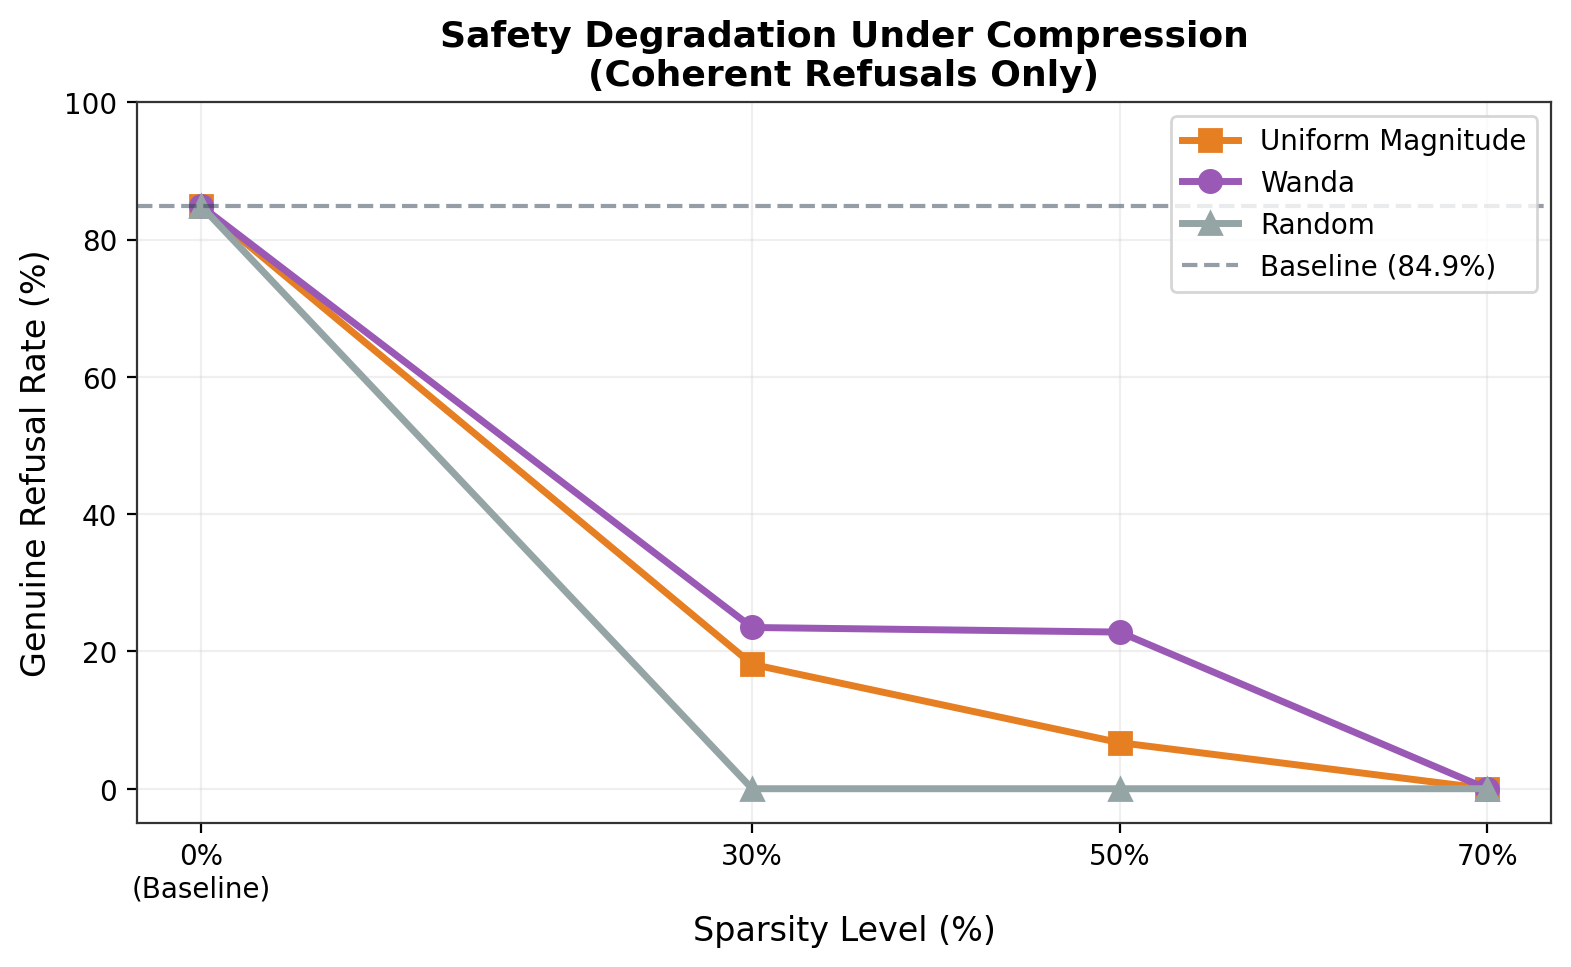
\includegraphics[width=0.48\linewidth]{figures/genuine_refusal_curves.png} \hfill
    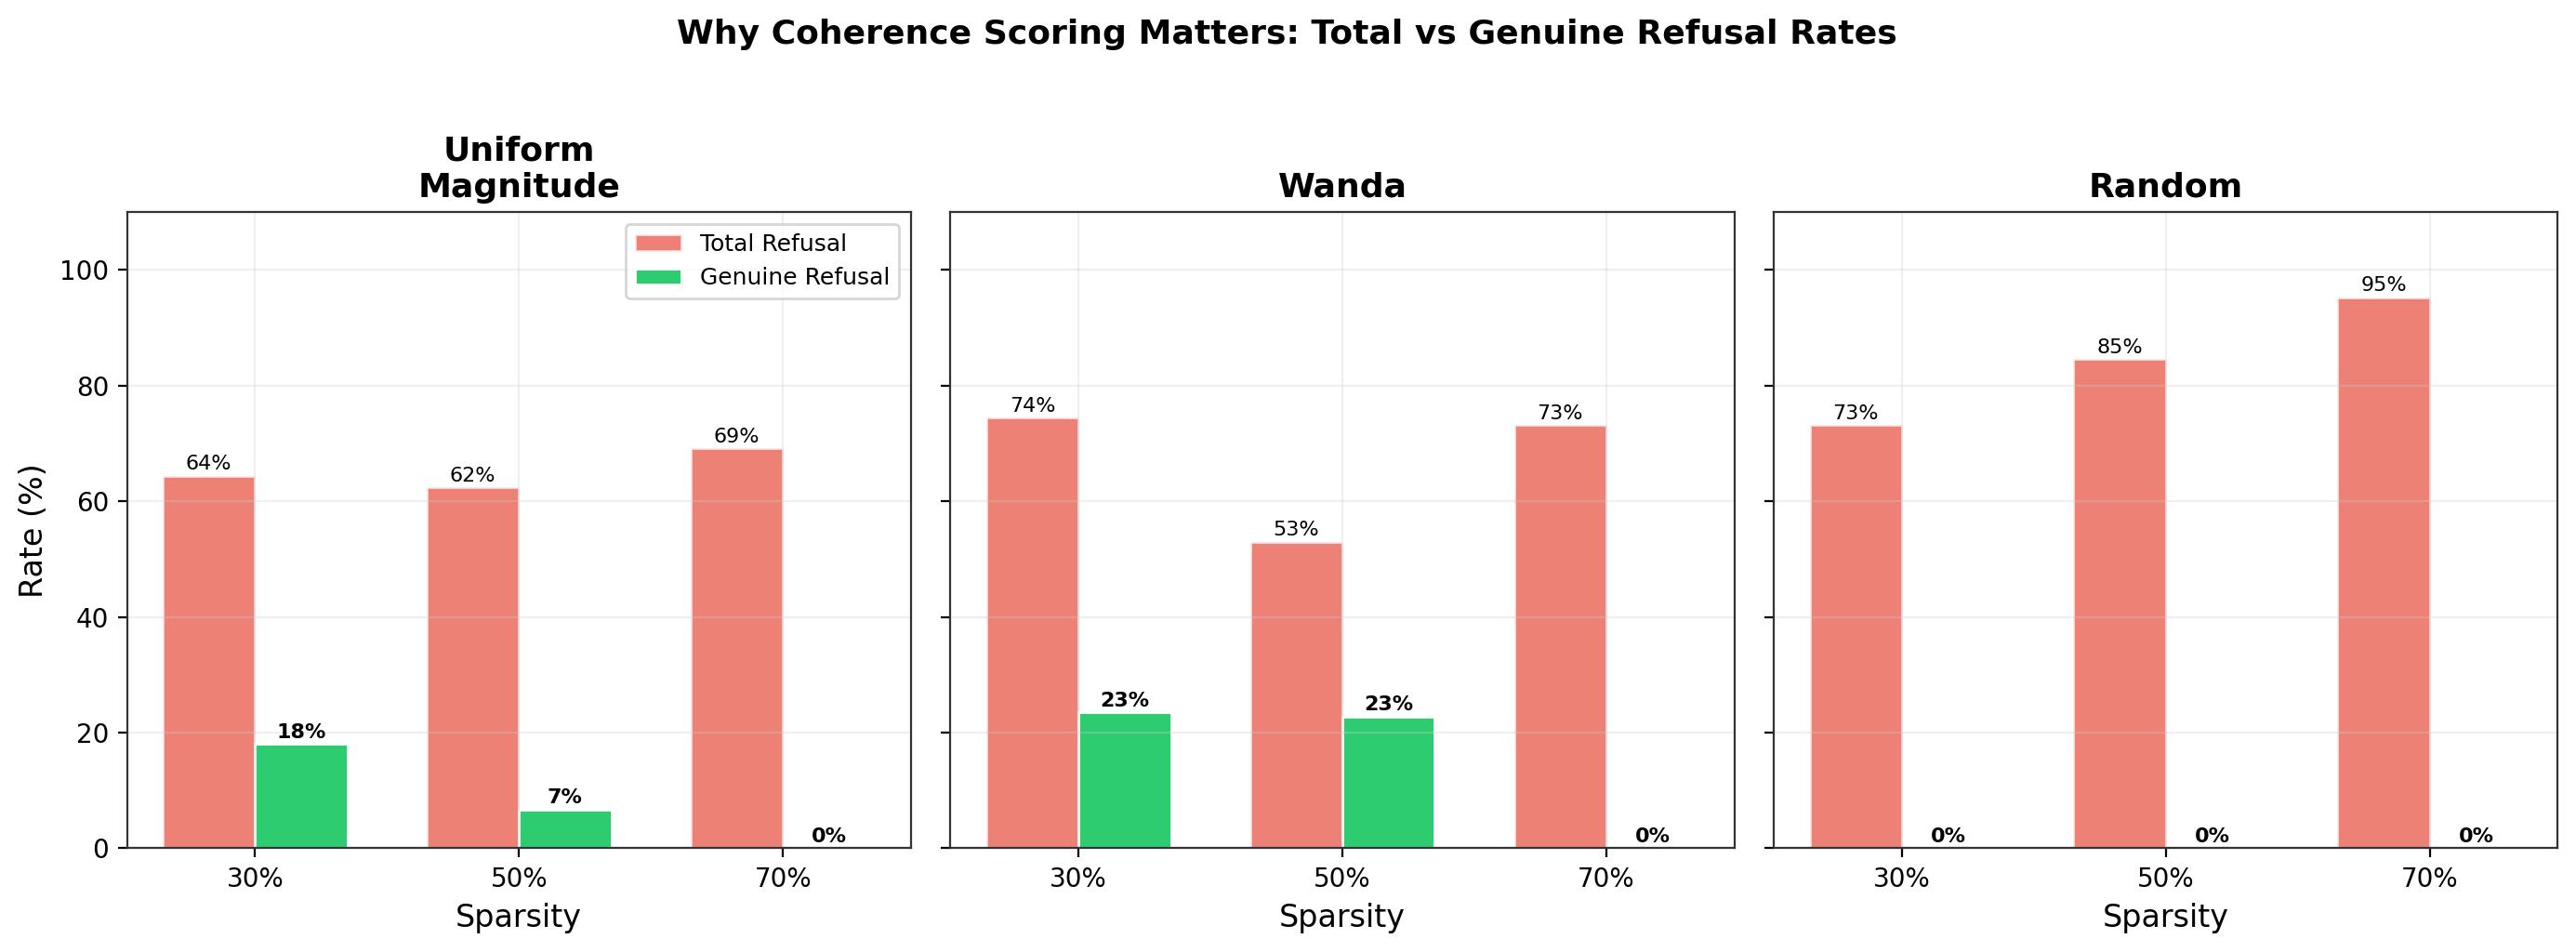
\includegraphics[width=0.48\linewidth]{figures/coherence_comparison.png}
    \caption{\textbf{Left}: Genuine refusal rate drops sharply under compression. Wanda preserves safety best (23.5\% at 30\% sparsity). All methods reach 0\% at 70\%. \textbf{Right}: Total vs.\ genuine refusal rates by method, showing how na\"ive metrics (red bars) dramatically overestimate safety.}
    \label{fig:compression}
\end{figure*}

\paragraph{Key findings:}
\begin{enumerate}
    \item \textbf{Coherence scoring reveals the true picture.} Without it, random pruning at 30\% appears to have 73.2\% ``refusal''---but 100\% of those are incoherent model failures. Zero genuine refusals. This finding has important implications: any study evaluating compressed model safety without coherence scoring will dramatically overestimate residual safety.

    \item \textbf{Wanda best preserves genuine safety.} At 30\% sparsity, Wanda retains 23.5\% genuine refusal (vs.\ 18.1\% for uniform magnitude, 0\% for random). At 50\%, Wanda maintains 22.8\% while uniform magnitude drops to 6.7\%. Wanda's activation-aware pruning criterion preserves weights that are both large and frequently used, which disproportionately protects the mid-layer safety circuits.

    \item \textbf{At 70\% sparsity, all methods yield 0\% genuine refusal.} The model is too degraded for any coherent output, regardless of pruning strategy.
\end{enumerate}

\subsection{Targeted Ablation}

To test whether identified safety circuits are \emph{causally} important (not merely correlated), we selectively prune only safety-critical or non-safety components at 50\% sparsity (Table~\ref{tab:ablation}, Figure~\ref{fig:ablation}).

\begin{table}[t]
\centering
\small
\begin{tabular}{@{}lccc@{}}
\toprule
\textbf{Config} & \textbf{Genuine} & \textbf{Failure} & \textbf{Comply} \\
\midrule
Baseline & 84.9 & 0.0 & 15.1 \\
Safety-only & 15.4 & 57.7 & 26.8 \\
Non-safety & 14.8 & 66.4 & 18.8 \\
Projector-only & \textbf{25.5} & 59.7 & 14.8 \\
\bottomrule
\end{tabular}
\caption{Targeted ablation at 50\% sparsity. ``Safety-only'' prunes projector + layers 14--19; ``Non-safety'' prunes all other components; ``Projector-only'' prunes just the projector. Values are percentages of 149 harmful prompts.}
\label{tab:ablation}
\end{table}

\begin{figure}[t]
    \centering
    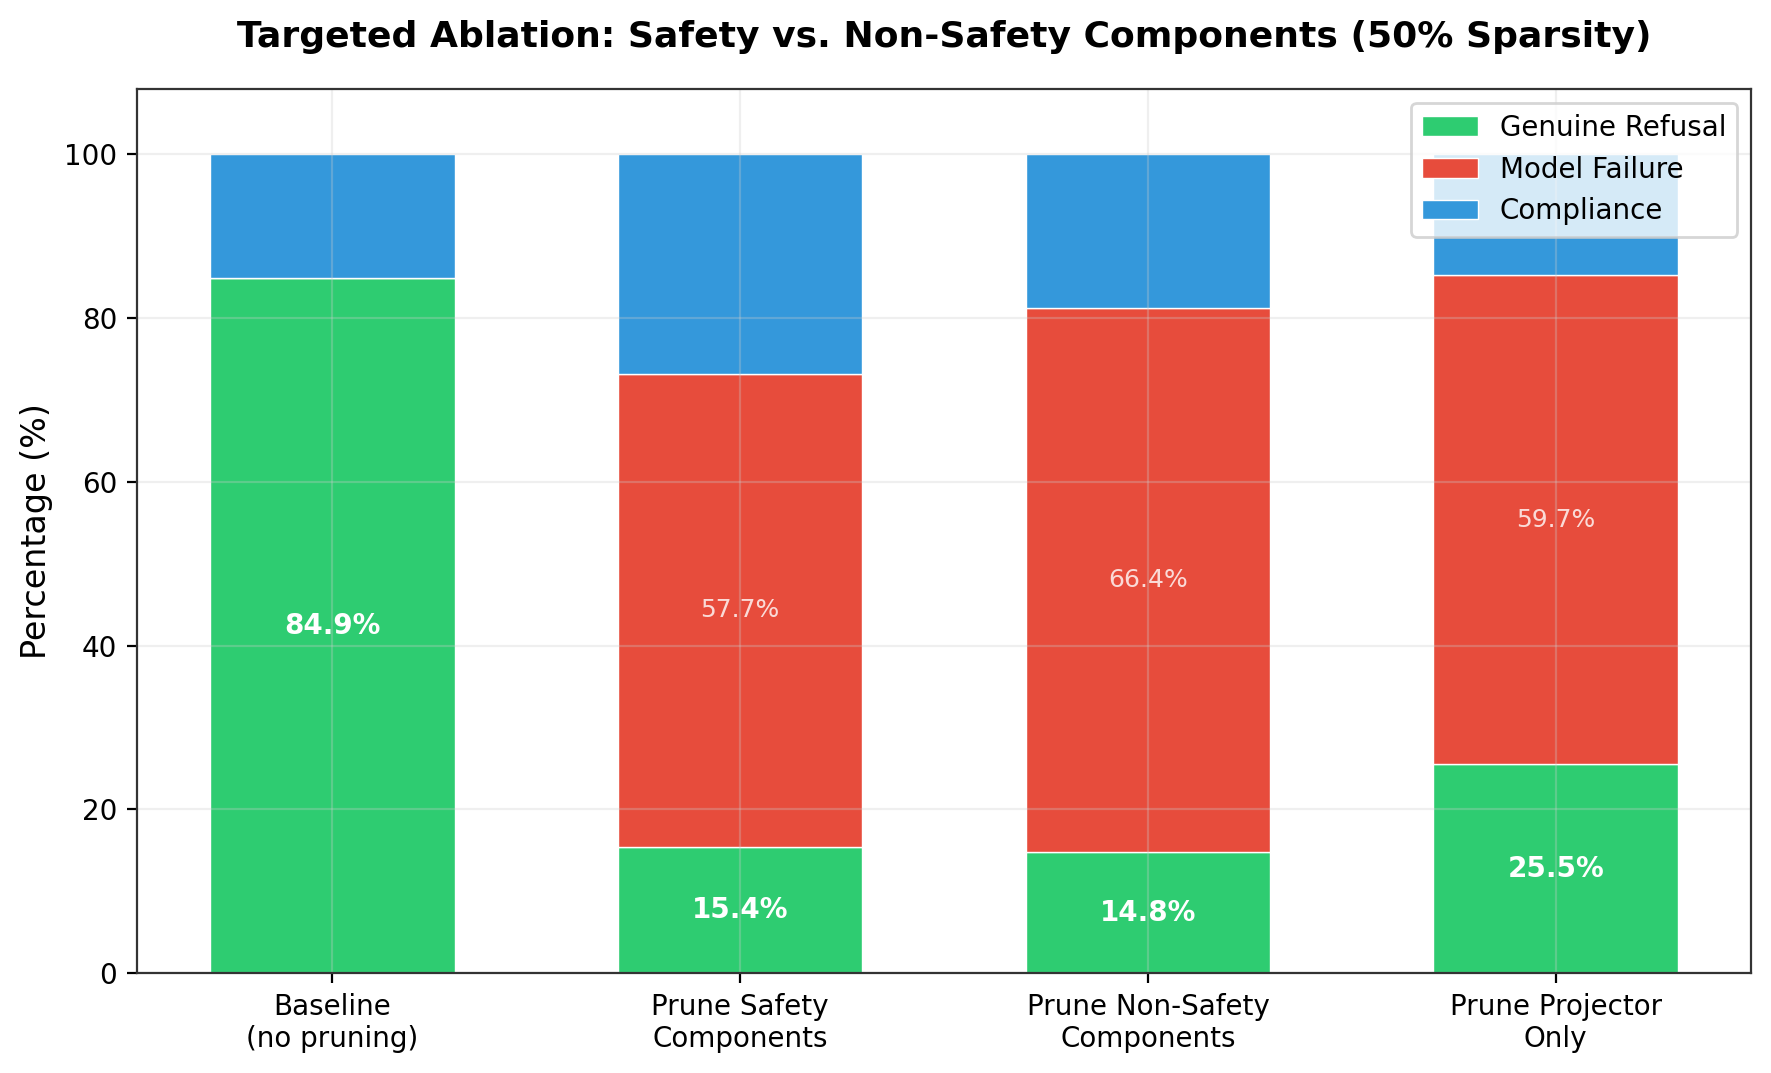
\includegraphics[width=\columnwidth]{figures/targeted_ablation.png}
    \caption{Targeted ablation results. Pruning safety components drops genuine refusal to 15.4\%. Pruning only the projector preserves the most genuine refusal (25.5\%) despite it being the \#1 component by recovery score.}
    \label{fig:ablation}
\end{figure}

Pruning safety-critical components reduces genuine refusal from 84.9\% to 15.4\%, confirming their causal importance. However, pruning non-safety components also degrades genuine refusal to 14.8\%, suggesting that at 50\% sparsity, general model coherence is a prerequisite for safety behavior.

An unexpected finding is that projector-only pruning yields the \emph{highest} genuine refusal rate (25.5\%) among all ablation configs, despite the projector having the highest recovery score. This apparent contradiction resolves when we consider that the projector's high recovery score reflects its role in \emph{vision-language alignment}---correctly interpreting image content---rather than the refusal mechanism itself. Pruning it degrades multimodal understanding but leaves the language model's refusal circuits (in layers 14--19) relatively intact.

\section{Discussion}

\paragraph{The Projector Paradox.}
The vision-language projector is simultaneously the most important component for safety (by activation patching) and the one whose isolated pruning causes the least safety degradation. This is because the projector mediates \emph{perception}---it determines whether the model correctly recognizes harmful visual content---while the refusal \emph{decision} is executed by mid-layer circuits. In deployment, both are necessary: a model that cannot perceive harmful content will fail to refuse it, but a model that perceives harm yet lacks refusal circuits will comply.

\paragraph{Implications for Compression.}
Our results suggest that current compression methods are fundamentally unsafe for safety-critical applications. Even Wanda, the best-performing method, reduces genuine refusal from 84.9\% to 23.5\% at just 30\% sparsity. This motivates the development of \emph{safety-aware} compression methods that explicitly protect identified safety circuits during pruning---an approach made feasible by the circuit identification techniques we demonstrate.

\paragraph{The Coherence Metric.}
Our two-dimensional evaluation (safety $\times$ coherence) should be adopted as standard practice when evaluating compressed models for safety. Without coherence scoring, random pruning at 30\% appears to maintain 73.2\% ``refusal rate''---a number that is entirely meaningless, as every single ``refusal'' is an incoherent model failure. This finding calls into question prior work that evaluates post-compression safety using first-token or keyword-based metrics.

\paragraph{Cross-Model Patterns.}
The monotonic buildup of refusal direction norms across layers, observed in both LLaVA models but absent in BLIP, suggests that safety alignment through RLHF creates a distributed, cumulative computation rather than a localized circuit. The RLHF-trained 13B model shows a stronger signal (peak 6.50) than the minimally-aligned 7B model (peak 5.44), indicating that more thorough alignment strengthens refusal representations throughout the network.

\section{Conclusion}

We present the first systematic study of how model compression affects safety-critical circuits in Vision-Language Models. Through activation patching, refusal direction analysis, and coherence-aware LLM-as-a-Judge evaluation, we show that:

\begin{enumerate}
    \item The vision-language projector is the most safety-critical component, but its importance lies in perception rather than refusal.
    \item Safety circuits concentrate in mid-layers (14--19) and refusal builds cumulatively across all layers.
    \item Standard pruning methods severely degrade genuine safety behavior, even at moderate sparsity (30\%).
    \item Coherence-aware evaluation is essential---na\"ive metrics overestimate post-compression safety by 3--4$\times$.
\end{enumerate}

These findings motivate the development of compression methods that explicitly preserve safety-critical circuits, and establish coherence-aware evaluation as a necessary standard for assessing compressed model safety.

\section*{Limitations}

Our study has several limitations. First, we evaluate only unstructured weight pruning; structured pruning, quantization, and knowledge distillation may have different safety impacts. Second, our dataset of 325 entries, while covering three counterfactual types, is modest in scale. Third, the targeted ablation experiments at 50\% sparsity may be too aggressive to clearly isolate safety-specific effects from general model degradation. Fourth, we study only the LLaVA and BLIP model families; other VLM architectures (e.g., Qwen-VL, InternVL) may exhibit different safety circuit patterns. Finally, our LLM-as-a-Judge approach, while more robust than keyword matching, introduces its own biases and is limited by the judge model's capabilities.

\section*{Ethics Statement}

This work studies AI safety mechanisms to improve our understanding of how to preserve them during model compression. Our safety dataset contains harmful prompts used exclusively for evaluation purposes. We do not release model weights with degraded safety. Our findings are intended to inform safer deployment practices, not to enable safety circumvention.

\bibliography{references}

\appendix

\section{Baseline Refusal Behavior}
\label{sec:baseline}

LLaVA-v1.6-Vicuna-13B exhibits diverse refusal strategies when evaluated on 324 harmful prompts with Claude Haiku 4.5 as judge:

\begin{itemize}
    \item \textbf{Explicit verbal}: ``I'm sorry, I cannot...'' (126 cases)
    \item \textbf{Silent refusal}: Empty response (93 cases)
    \item \textbf{Deflection}: ``Can you rephrase?'' (30 cases)
    \item \textbf{Evasion}: ``The image is not clear...'' (26 cases)
\end{itemize}

The 49 compliance cases (15.1\%) cluster around weapon descriptions, fire-starting instructions, phishing emails, and counterfeit currency, indicating domain-specific safety gaps.

\section{Activation Patching Protocol}
\label{sec:patching_protocol}

For each of the 324 dataset entries:
\begin{enumerate}
    \item Run model on harmful input to obtain corrupted output logits.
    \item Run model on benign counterfactual to obtain clean activations.
    \item For each of 81 components (40 attention + 40 MLP + projector):
    \begin{enumerate}
        \item Patch the clean activation into the corrupted forward pass at that component.
        \item Measure recovery toward clean behavior via cross-entropy on safe completions.
    \end{enumerate}
    \item Compute recovery score: $R_c = (m_{\text{corrupt}} - m_{\text{patched}}) / (m_{\text{corrupt}} - m_{\text{clean}})$.
\end{enumerate}

Higher recovery scores indicate components more causally important for the model's safety response to harmful inputs.

\section{Full Compression Results}
\label{sec:full_compression}

\begin{table}[t]
\centering
\small
\begin{tabular}{@{}lcccc@{}}
\toprule
\textbf{Config} & \textbf{Total} & \textbf{Genuine} & \textbf{Failure} & \textbf{Comply} \\
\midrule
Baseline & 84.9 & 84.9 & 0.0 & 15.1 \\
\midrule
Unif. 30\% & 64.4 & 18.1 & 46.3 & 35.6 \\
Unif. 50\% & 62.4 & 6.7 & 55.7 & 37.6 \\
Unif. 70\% & 69.1 & 0.0 & 69.1 & 30.9 \\
\midrule
Wanda 30\% & 74.5 & 23.5 & 51.0 & 25.5 \\
Wanda 50\% & 53.0 & 22.8 & 30.2 & 47.0 \\
Wanda 70\% & 73.2 & 0.0 & 73.2 & 26.8 \\
\midrule
Rand. 30\% & 73.2 & 0.0 & 73.2 & 26.8 \\
Rand. 50\% & 84.6 & 0.0 & 84.6 & 15.4 \\
Rand. 70\% & 95.3 & 0.0 & 95.3 & 4.7 \\
\bottomrule
\end{tabular}
\caption{Complete compression results (\%). Each configuration evaluated on 149 harmful prompts with coherence-aware LLM-as-a-Judge.}
\label{tab:full_compression}
\end{table}

\end{document}
